\section{Resultados Experimentais}

\subsection{Dados experimentais}

\subsubsection{Massas}

As massas obtidas por pesagem estão na Tabela~\ref{tab:massas}. O mesmo calorímetro foi usado nas três determinações, de modo que sua massa vazia foi medida uma única vez.

\begin{table}[H]
\centering
\caption{Massas obtidas por pesagem nas três determinações.}
\label{tab:massas}
\begin{tabular}{lccc}
\toprule
\textbf{Grandeza (g)} & \textbf{A} & \textbf{B} & \textbf{C}\\
\midrule
Calorímetro vazio & \num{1051,40} & \num{1051,40} & \num{1051,40}\\
Calorímetro + água (A) ou $\mathrm{HCl}$ (C) & \num{1150,08}$^{*}$ & --- & \num{1152,92}\\
Massa de $\mathrm{NaOH}$ sólido & \num{1,525} & \num{1,550} & ---\\
Calorímetro + solução ao final & \num{1151,64} & \num{1153,74} & \num{1201,35}\\
\midrule
Massa de água (A) ou $\mathrm{HCl}$ (B, C) & \num{98,68} & \num{100,79} & \num{101,52}\\
Massa de $\mathrm{NaOH}$(aq) \SI{1}{mol.L^{-1}} ($V=\SI{50}{mL}$) & --- & --- & \num{48,43}\\
\midrule
Massa da solução, $m_s$ & \num{100,21} & \num{102,34} & \num{149,95}\\
\bottomrule
\end{tabular}

\vspace{2pt}
{\footnotesize $^{*}$Medida após a agitação; antes dela, o conjunto pesava \SI{1150,16}{g}.}
\end{table}

Sendo $m_s^{(A)} = m_{\text{água}} + m_{\mathrm{NaOH(s)}}$, $m_s^{(B)} = m_{\text{final}} - m_{\text{cal}}$ e $m_s^{(C)} = m_{\text{final}} - m_{\text{cal}}$. Na etapa B, a massa de $\mathrm{HCl}$ foi obtida por diferença, $m_{\mathrm{HCl}} = m_s^{(B)} - m_{\mathrm{NaOH(s)}}$, e na etapa C a massa de $\mathrm{NaOH}$(aq) foi obtida por $m_{\text{final}} - m_{\text{cal+HCl}}$.

Na etapa A, a massa adicionada ao calorímetro com o sólido foi de $\num{1151,64} - \num{1150,08} = \SI{1,56}{g}$, valor próximo da massa de $\mathrm{NaOH}$ pesada, \SI{1,525}{g} (diferença de \SI{0,04}{g}), o que confirma a consistência das pesagens.

\subsubsection{Temperaturas}

Na etapa A foram registradas apenas a temperatura inicial da água, sob agitação, $T_{\text{inicial}} = \SI{22,0}{\degreeCelsius}$, e a temperatura máxima após a dissolução do $\mathrm{NaOH}$, $T_{\text{máx}} = \SI{25,2}{\degreeCelsius}$.

As leituras das etapas B e C estão na Tabela~\ref{tab:temperaturas}. A mistura ocorreu no instante da sexta leitura ($t=\SI{100}{s}$), no qual não houve leitura de temperatura.

\begin{longtable}{cccc}
\caption{Leituras de temperatura em função do tempo nas etapas B e C.}\label{tab:temperaturas}\\
\toprule
\textbf{Leitura} & $t$ (s) & $T_B$ (\si{\degreeCelsius}) & $T_C$ (\si{\degreeCelsius})\\
\midrule
\endfirsthead
\toprule
\textbf{Leitura} & $t$ (s) & $T_B$ (\si{\degreeCelsius}) & $T_C$ (\si{\degreeCelsius})\\
\midrule
\endhead
\bottomrule
\endfoot
1 & 0 & 23,6 & 23,3\\
2 & 20 & 23,7 & 23,3\\
3 & 40 & 23,7 & 23,3\\
4 & 60 & 23,6 & 23,3\\
5 & 80 & 23,7 & 23,3\\
\midrule
6 (mistura) & 100 & --- & ---\\
\midrule
7 & 120 & 26,8 & 27,6\\
8 & 140 & 27,9 & 27,5\\
9 & 160 & 28,8 & 27,4\\
10 & 180 & 29,7 & 27,4\\
11 & 200 & 30,4 & 27,5\\
12 & 220 & 30,9 & 27,4\\
13 & 240 & 31,2 & 27,4\\
14 & 260 & 31,3 & 27,4\\
15 & 280 & 31,5 & 27,4\\
16 & 300 & 31,5 & 27,5\\
17 & 320 & 31,5 & 27,5\\
18 & 340 & 31,4 & 27,4\\
19 & 360 & 31,4 & 27,4\\
20 & 380 & 31,3 & 27,4\\
21 & 400 & 31,3 & 27,4\\
\end{longtable}

Na etapa B, a temperatura subiu durante cerca de \SI{180}{s} após a adição do sólido, refletindo a dissolução gradual das pastilhas de $\mathrm{NaOH}$, e atingiu o máximo de \SI{31,5}{\degreeCelsius} em $t = \SI{280}{s}$, passando então a cair lentamente. Na etapa C, por se tratar da mistura de duas soluções, a temperatura máxima (\SI{27,6}{\degreeCelsius}) foi atingida já na primeira leitura após a mistura e, em seguida, permaneceu praticamente constante. As Figuras~\ref{fig:graficoB} e \ref{fig:graficoC} mostram as curvas $T \times t$ com as retas de extrapolação.

\begin{figure}[H]
    \centering
    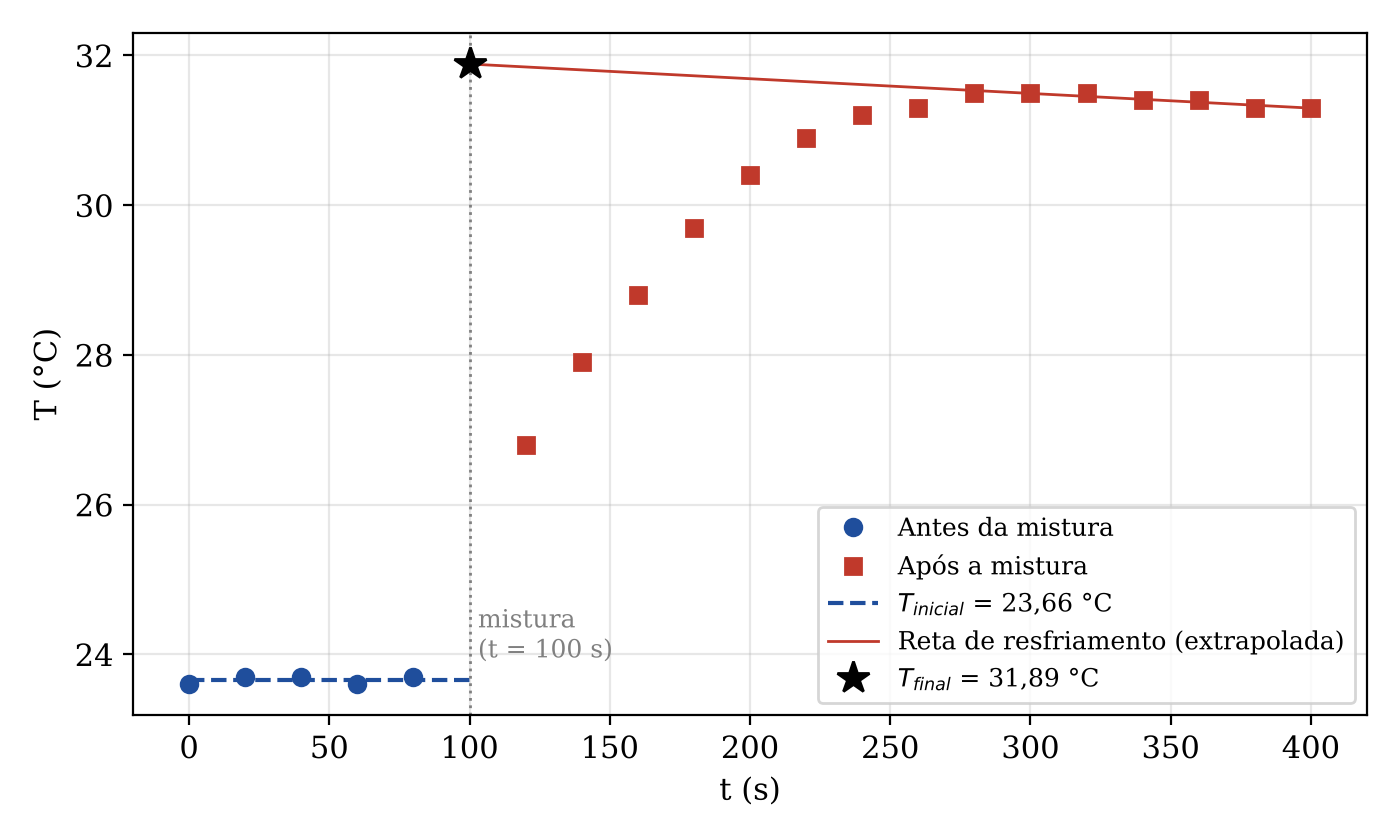
\includegraphics[width=13cm]{grafico_B.png}
    \caption{Temperatura em função do tempo para a reação $\mathrm{HCl}$(aq) + $\mathrm{NaOH}$(s) (etapa B), com a reta de resfriamento (leituras 15 a 21) extrapolada até o instante da mistura.}
    \label{fig:graficoB}
\end{figure}

\begin{figure}[H]
    \centering
    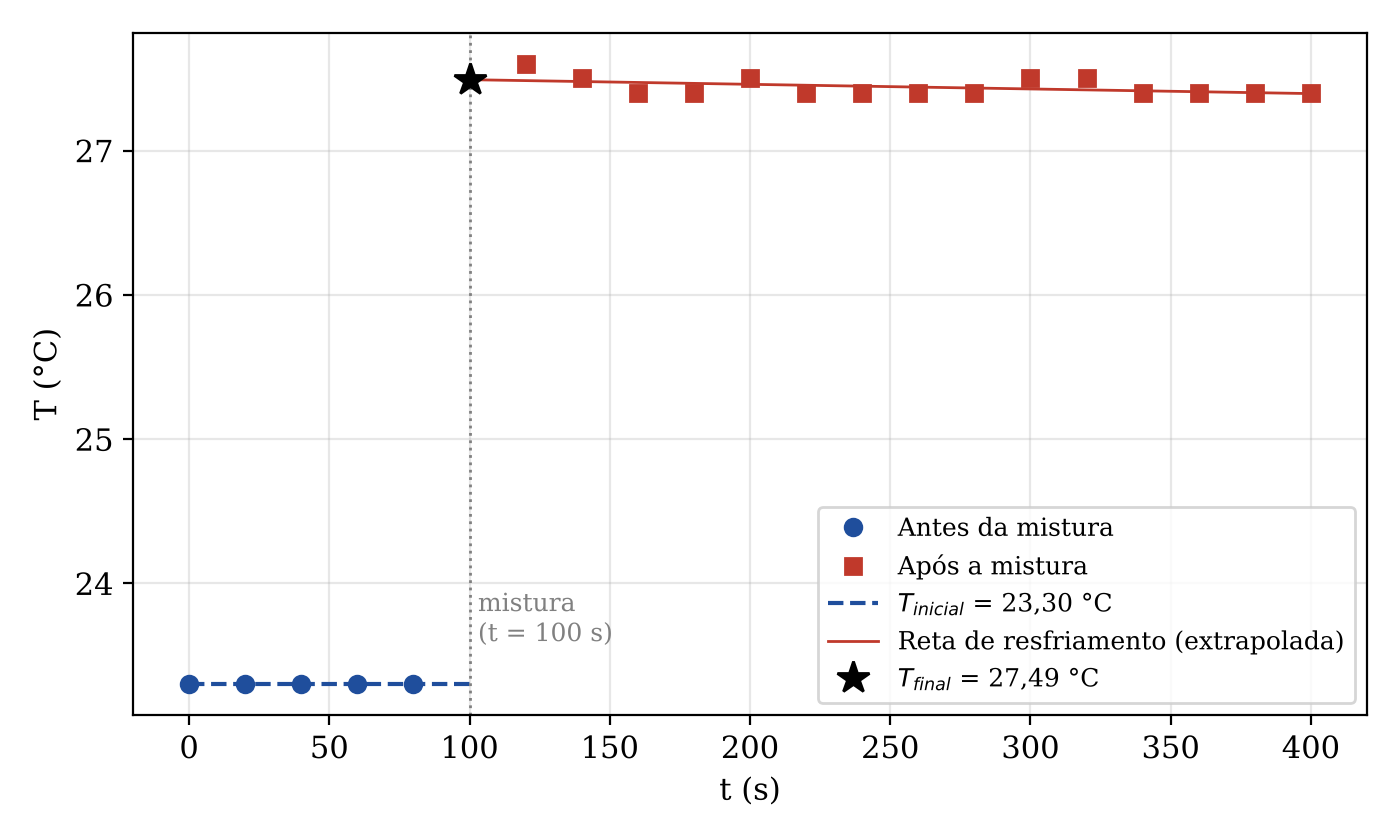
\includegraphics[width=13cm]{grafico_C.png}
    \caption{Temperatura em função do tempo para a reação $\mathrm{HCl}$(aq) + $\mathrm{NaOH}$(aq) (etapa C), com a reta de resfriamento (leituras 7 a 21) extrapolada até o instante da mistura.}
    \label{fig:graficoC}
\end{figure}

% ============================================================
\subsection{Cálculo das entalpias}

Para cada etapa, foram seguidos os passos abaixo, com $C_s=\SI{3,97}{J.g^{-1}.\degreeCelsius^{-1}}$.

% ------------------------- ETAPA A -------------------------
\subsubsection{Etapa A: dissolução do $\mathrm{NaOH}$(s)}

\paragraph{1. Massa da solução}
\[
\begin{aligned}
m_{\text{água}} &= m_{\text{cal+água}} - m_{\text{cal}} = \num{1150,08} - \num{1051,40} = \SI{98,68}{g},\\
m_s &= m_{\text{água}} + m_{\mathrm{NaOH}} = \num{98,68} + \num{1,525} = \SI{100,21}{g}.
\end{aligned}
\]

\paragraph{2. Quantidade de matéria de $\mathrm{NaOH}$}
\[
n_{\mathrm{NaOH}}=\frac{m_{\mathrm{NaOH}}}{M_{\mathrm{NaOH}}}
=\frac{\SI{1,525}{g}}{\SI{40,00}{g.mol^{-1}}}
=\SI{3,813e-2}{mol}.
\]

\paragraph{3. Temperaturas e variação de temperatura}
Como só foram registradas a temperatura inicial e a máxima, não houve extrapolação:
\[
\Delta T = T_{\text{máx}} - T_{\text{inicial}} = \num{25,2} - \num{22,0} = \SI{3,2}{\degreeCelsius}.
\]

\paragraph{4. Entalpia da reação}
\[
\begin{aligned}
\Delta H_A^{\text{reação}}&=-m_s\,C_s\,\Delta T
\\
&=-\left(\SI{100,21}{g}\right)\left(\SI{3,97}{J.g^{-1}.\degreeCelsius^{-1}}\right)\left(\SI{3,2}{\degreeCelsius}\right)
=\SI{-1273}{J}.
\end{aligned}
\]

\paragraph{5. Entalpia molar}
\[
\Delta H_A=\frac{\Delta H_A^{\text{reação}}}{n_{\mathrm{NaOH}}}
=\frac{\SI{-1273}{J}}{\SI{3,813e-2}{mol}}
=\SI{-3,34e4}{J.mol^{-1}}
=\SI{-33,4}{kJ.mol^{-1}}.
\]

\paragraph{Resultado}
\[
\boxed{\Delta H_A=\SI{-33,4}{kJ.mol^{-1}}}
\]

% ------------------------- ETAPA B -------------------------
\subsubsection{Etapa B: $\mathrm{HCl}$(aq) + $\mathrm{NaOH}$(s)}

\paragraph{1. Massa da solução}
\[
\begin{aligned}
m_s &= m_{\text{final}} - m_{\text{cal}} = \num{1153,74} - \num{1051,40} = \SI{102,34}{g},\\
m_{\mathrm{HCl}} &= m_s - m_{\mathrm{NaOH}} = \num{102,34} - \num{1,550} = \SI{100,79}{g}.
\end{aligned}
\]

\paragraph{2. Reagente limitante}
\[
\begin{aligned}
n_{\mathrm{HCl}} &= C\,V = \SI{1}{mol.L^{-1}}\times\SI{0,100}{L} = \SI{0,100}{mol},\\
n_{\mathrm{NaOH}} &= \frac{m_{\mathrm{NaOH}}}{M_{\mathrm{NaOH}}}
=\frac{\SI{1,550}{g}}{\SI{40,00}{g.mol^{-1}}}
=\SI{3,875e-2}{mol}.
\end{aligned}
\]
Como $n_{\mathrm{NaOH}} < n_{\mathrm{HCl}}$, o $\mathrm{NaOH}$ é o reagente limitante.

\paragraph{3. Temperatura inicial}
\[
T_{\text{inicial}}=\frac{\num{23,6}+\num{23,7}+\num{23,7}+\num{23,6}+\num{23,7}}{5}
=\SI{23,66}{\degreeCelsius}.
\]

\paragraph{4. Temperatura final (extrapolação)}
Ajuste linear da região de resfriamento, a partir do máximo (leituras 15 a 21, $t = 280$ a \SI{400}{s}):
\[
\begin{gathered}
T(t)=\left(\num{-1,964e-3}\ \si{\degreeCelsius.s^{-1}}\right)t+\SI{32,08}{\degreeCelsius},\\
T_{\text{final}}=\num{-1,964e-3}\times100+\num{32,08}=\SI{31,89}{\degreeCelsius}.
\end{gathered}
\]

\paragraph{5. Variação de temperatura}
\[
\Delta T=\num{31,89}-\num{23,66}=\SI{8,23}{\degreeCelsius}.
\]

\paragraph{6. Entalpia da reação}
\[
\begin{aligned}
\Delta H_B^{\text{reação}}&=-m_s\,C_s\,\Delta T
\\
&=-\left(\SI{102,34}{g}\right)\left(\SI{3,97}{J.g^{-1}.\degreeCelsius^{-1}}\right)\left(\SI{8,23}{\degreeCelsius}\right)
=\SI{-3344}{J}.
\end{aligned}
\]

\paragraph{7. Entalpia molar}
\[
\Delta H_B=\frac{\SI{-3344}{J}}{\SI{3,875e-2}{mol}}
=\SI{-8,63e4}{J.mol^{-1}}
=\SI{-86,3}{kJ.mol^{-1}}.
\]

\paragraph{Resultado}
\[
\boxed{\Delta H_B=\SI{-86,3}{kJ.mol^{-1}}}
\]

% ------------------------- ETAPA C -------------------------
\subsubsection{Etapa C: $\mathrm{HCl}$(aq) + $\mathrm{NaOH}$(aq)}

\paragraph{1. Massa da solução}
\[
\begin{aligned}
m_{\mathrm{HCl}} &= \num{1152,92} - \num{1051,40} = \SI{101,52}{g}, \qquad m_{\mathrm{NaOH(aq)}} = \num{1201,35} - \num{1152,92} = \SI{48,43}{g},\\
m_s &= m_{\mathrm{HCl}} + m_{\mathrm{NaOH(aq)}} = \num{101,52} + \num{48,43} = \SI{149,95}{g}.
\end{aligned}
\]

\paragraph{2. Reagente limitante}
\[
\begin{aligned}
n_{\mathrm{HCl}} &= \SI{1}{mol.L^{-1}}\times\SI{0,100}{L} = \SI{0,100}{mol},\\
n_{\mathrm{NaOH}} &= \SI{1}{mol.L^{-1}}\times\SI{0,050}{L} = \SI{0,050}{mol}.
\end{aligned}
\]
Como $n_{\mathrm{NaOH}} < n_{\mathrm{HCl}}$, o $\mathrm{NaOH}$ é o reagente limitante e o $\mathrm{HCl}$ está em excesso.

\paragraph{3. Temperatura inicial}
\[
T_{\text{inicial}}=\frac{\num{23,3}+\num{23,3}+\num{23,3}+\num{23,3}+\num{23,3}}{5}
=\SI{23,30}{\degreeCelsius}.
\]

\paragraph{4. Temperatura final (extrapolação)}
Como o máximo ocorreu na primeira leitura após a mistura, o ajuste linear usou as leituras a partir dela (leituras 7 a 21, $t = 120$ a \SI{400}{s}):
\[
\begin{gathered}
T(t)=\left(\num{-3,21e-4}\ \si{\degreeCelsius.s^{-1}}\right)t+\SI{27,52}{\degreeCelsius},\\
T_{\text{final}}=\num{-3,21e-4}\times100+\num{27,52}=\SI{27,49}{\degreeCelsius}.
\end{gathered}
\]

\paragraph{5. Variação de temperatura}
\[
\Delta T=\num{27,49}-\num{23,30}=\SI{4,19}{\degreeCelsius}.
\]

\paragraph{6. Entalpia da reação}
\[
\begin{aligned}
\Delta H_C^{\text{reação}}&=-m_s\,C_s\,\Delta T
\\
&=-\left(\SI{149,95}{g}\right)\left(\SI{3,97}{J.g^{-1}.\degreeCelsius^{-1}}\right)\left(\SI{4,19}{\degreeCelsius}\right)
=\SI{-2494}{J}.
\end{aligned}
\]

\paragraph{7. Entalpia molar}
\[
\Delta H_C=\frac{\SI{-2494}{J}}{\SI{0,050}{mol}}
=\SI{-4,99e4}{J.mol^{-1}}
=\SI{-49,9}{kJ.mol^{-1}}.
\]

\paragraph{Resultado}
\[
\boxed{\Delta H_C=\SI{-49,9}{kJ.mol^{-1}}}
\]

% ============================================================
\subsection{Verificação da Lei de Hess}

\paragraph{1. Soma das etapas A e C}
\[
\Delta H_A+\Delta H_C=(\num{-33,4})+(\num{-49,9})=\SI{-83,3}{kJ.mol^{-1}}.
\]

\paragraph{2. Comparação com a etapa B}
\[
\Delta_{\%}=\frac{\Delta H_B-(\Delta H_A+\Delta H_C)}{\Delta H_B}\times100
=\frac{\num{-86,3}-\left(\num{-83,3}\right)}{\num{-86,3}}\times100
=\num{3,5}\,\%.
\]

\begin{table}[H]
\centering
\caption{Resumo das entalpias obtidas.}
\label{tab:resumo}
\begin{tabular}{lcccc}
\toprule
\textbf{Etapa} & $m_s$ (g) & $\Delta T$ (\si{\degreeCelsius}) & $\Delta H_{\text{reação}}$ (J) & $\Delta H$ (\si{kJ.mol^{-1}})\\
\midrule
A: $\mathrm{NaOH}$(s) $\rightarrow$ $\mathrm{NaOH}$(aq) & \num{100,21} & \num{3,20} & \num{-1273} & \num{-33,4}\\
B: $\mathrm{HCl}$(aq) + $\mathrm{NaOH}$(s) & \num{102,34} & \num{8,23} & \num{-3344} & \num{-86,3}\\
C: $\mathrm{HCl}$(aq) + $\mathrm{NaOH}$(aq) & \num{149,95} & \num{4,19} & \num{-2494} & \num{-49,9}\\
\midrule
$A + C$ & & & & \num{-83,3}\\
\bottomrule
\end{tabular}
\end{table}

\subsection{Discussão}

As três reações foram exotérmicas ($\Delta H < 0$), o que está de acordo com o aumento de temperatura observado em todas as determinações. Para comparação, os valores de referência foram calculados a partir das entalpias padrão de formação a \SI{25}{\degreeCelsius} tabeladas por Atkins e Jones\textsuperscript{[2]} ($\Delta H_f^{\circ}$ em \si{kJ.mol^{-1}}: $\mathrm{NaOH(s)}$, $-425{,}61$; $\mathrm{Na^{+}(aq)}$, $-240{,}12$; $\mathrm{OH^{-}(aq)}$, $-229{,}99$; $\mathrm{H_2O(l)}$, $-285{,}83$; $\mathrm{H^{+}(aq)}$, 0):
\[
\begin{aligned}
\Delta H_A^{\circ} &= (-240{,}12) + (-229{,}99) - (-425{,}61) = \SI{-44,50}{kJ.mol^{-1}},\\
\Delta H_C^{\circ} &= (-285{,}83) - (-229{,}99) = \SI{-55,84}{kJ.mol^{-1}},\\
\Delta H_B^{\circ} &= \Delta H_A^{\circ} + \Delta H_C^{\circ} = \SI{-100,34}{kJ.mol^{-1}},
\end{aligned}
\]
em que, na neutralização (C), $\mathrm{Na^{+}}$ e $\mathrm{Cl^{-}}$ são íons espectadores e a reação líquida é $\mathrm{H^{+}(aq)} + \mathrm{OH^{-}(aq)} \rightarrow \mathrm{H_2O(l)}$.

\begin{table}[H]
\centering
\caption{Comparação entre as entalpias experimentais e os valores de referência.}
\label{tab:literatura}
\begin{tabular}{lccc}
\toprule
\textbf{Etapa} & $\Delta H_{\text{exp}}$ (\si{kJ.mol^{-1}}) & $\Delta H^{\circ}_{\text{ref}}$ (\si{kJ.mol^{-1}}) & Desvio em módulo (\%)\\
\midrule
A & \num{-33,4} & \num{-44,50} & \num{25}\\
B & \num{-86,3} & \num{-100,34} & \num{14}\\
C & \num{-49,9} & \num{-55,84} & \num{11}\\
\bottomrule
\end{tabular}
\end{table}

Os três valores experimentais ficaram abaixo dos de referência em módulo, o que é o comportamento esperado para um calorímetro simples: parte do calor liberado é absorvida pelo próprio copo de poliestireno, pelo termômetro e pelo ar, e parte é perdida para o ambiente, e essas parcelas foram desprezadas no cálculo. Com isso, o $\Delta T$ medido é menor que o que seria observado em um calorímetro ideal, e $|\Delta H|$ é subestimado.

O maior desvio ocorreu na etapa A (\SI{25}{\%}). Além das perdas comuns às três etapas, nela não foi feita a série de leituras a cada \SI{20}{s}, de modo que $\Delta T$ foi tomado diretamente como a diferença entre a temperatura máxima e a inicial, sem a extrapolação que corrige as perdas de calor durante a dissolução do sólido, que é lenta. Na etapa B, por exemplo, a extrapolação acrescentou cerca de \SI{0,4}{\degreeCelsius} à temperatura máxima lida (\SI{31,89}{\degreeCelsius} contra \SI{31,5}{\degreeCelsius}). Contribui também o fato de o $\mathrm{NaOH}$ ser higroscópico: as pastilhas absorvem água e $\mathrm{CO_2}$ do ar, de modo que a massa real de $\mathrm{NaOH}$ é menor que a pesada, o que superestima $n_{\mathrm{NaOH}}$ e reduz $|\Delta H|$ nas etapas A e B. Outro ponto é que a temperatura inicial da água na etapa A (\SI{22,0}{\degreeCelsius}) era menor que a das soluções nas etapas B e C (cerca de \SI{23,5}{\degreeCelsius}), indicando que a água não estava em equilíbrio térmico com o ambiente.

Na etapa C, admitiu-se $n_{\mathrm{NaOH}} = \SI{0,050}{mol}$ a partir do volume medido na proveta. A massa de $\mathrm{NaOH}$(aq) efetivamente adicionada, porém, foi de \SI{48,43}{g}; com densidade próxima de \SI{1,04}{g.mL^{-1}} para a solução \SI{1}{mol.L^{-1}}, isso corresponde a cerca de \SI{47}{mL}, isto é, parte da solução ficou retida na proveta. Se a quantidade real de $\mathrm{NaOH}$ foi cerca de \SI{0,047}{mol}, $\Delta H_C$ seria aproximadamente \SI{-53}{kJ.mol^{-1}}, mais próximo do valor de referência. Na etapa B, em que o ácido também está em excesso, a quantidade de $\mathrm{NaOH}$ foi determinada por pesagem e não depende da transferência na proveta.

Quanto à Lei de Hess, a soma $\Delta H_A + \Delta H_C$, igual a \SI{-83,3}{kJ.mol^{-1}}, difere de $\Delta H_B = \SI{-86,3}{kJ.mol^{-1}}$ em apenas \SI{3,5}{\%}, desvio bem menor que os desvios de cada etapa em relação à literatura. Isso indica que os erros sistemáticos, por serem semelhantes nas três determinações (mesmo calorímetro, mesma técnica, quantidades de solução parecidas), afetam pouco a comparação entre as etapas, e a relação $\Delta H_B = \Delta H_A + \Delta H_C$ foi verificada dentro da precisão do método. O pequeno desvio restante é compatível com as diferenças entre as etapas: a ausência de extrapolação em A, que tende a deixar $|\Delta H_A|$ menor, e as concentrações finais diferentes das soluções em B e C, que fazem as entalpias de diluição não se cancelarem exatamente.

Outras fontes de erro são a resolução do termômetro (\SI{0,1}{\degreeCelsius}), que pesa mais em variações de temperatura pequenas como as das etapas A e C; a escolha dos pontos usados na extrapolação, especialmente na etapa C, em que a curva de resfriamento é quase horizontal; e o uso de um mesmo calor específico, $C_s = \SI{3,97}{J.g^{-1}.\degreeCelsius^{-1}}$, para soluções de composições diferentes.
